\chapter{EXPERIMENTAL SETTING, RESULTS AND DISCUSSION}
\label{sec:exp}
\section{Experimental Setting}
The proposed framework for aging tolerance is implemented in C++ and the SAT-based formulation is solved by MiniSat on a 2.83GHz Intel Quad-Core CPU workstation running Linux. The benchmark circuits are chosen from the IWLS'05 and ISCAS'89 suites. The technology used is TSMC 45nm GP standard cell series.

Under 10-year BTI, the aging rates of clock buffers were obtained from HSPICE. The aging rates of clock buffers with duty cycles of 20\%, 40\%, 50\%, and 80\% are 8.51\%, 12.08\%, 13.51\%, and 16.41\% respectively and the aging rate of logic is obtained by using the predictive model presented in~\cite{wang2010impact, wang2007efficient, gomez2016early, amrouch2016reliability} (detailed in Section~\ref{subsec:apm}).


\begin{table*}
\centering
\caption{Benchmark information}
	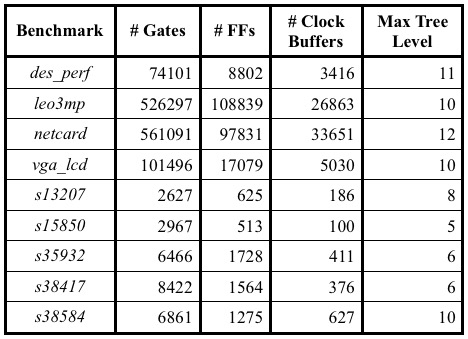
\includegraphics[width=0.7\columnwidth]{images/benchmark.png} 
\label{table:exp1}
\end{table*}
\begin{table*}
\centering
\caption{Results of aging tolerance}
	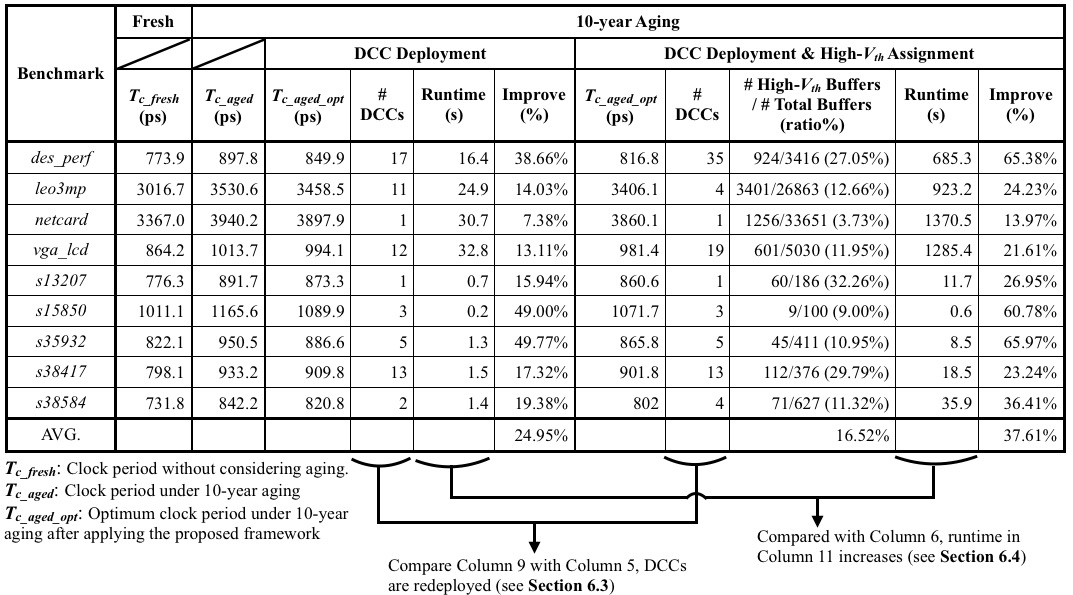
\includegraphics[width=1.1\columnwidth]{images/Experimental_result_DCC_TVA.png} 
\label{table:exp2}
\end{table*}
\section{Experimental Results}
Table~\ref{table:exp1} and Table~\ref{table:exp2} reports the information of each benchmark and the experimental results. In Table~\ref{table:exp1}, Columns 2 to 5 show the total count of gates, total count of flip-flops, total count of clock buffers, and maximum level of the clock tree in each benchmark respectively. In Table~\ref{table:exp2}, Column 4 to 7 show the results when DCC deployment is considered in the framework. Column 8 to 12 show the results when high-$V_{th}$ assignment for clock buffers is applied on top of DCC deployment.

In Table~\ref{table:exp2}, Column 2  demonstrates the fresh clock period that is the circuit delay without aging, denoted by $T_{c\_fresh}$. Column 3 demonstrates the clock period of the circuit under 10-year aging, denoted by $T_{c\_aged}$. Column 4 and 8 demonstrate the optimum clock period of the circuit under 10-year aging after applying our framework, denoted by $T_{c\_aged\_opt}$. A shorter clock period under aging implies better circuit performance and higher level of aging tolerance. Column 5 and 9 demonstrate the used DCC count. Column 6 and 11 demonstrate the runtime and the Column 7 and 12 demonstrate the improvement, i.e., the level of aging tolerance which is calculated as:
\begin{gather*}
1 - (T_{c\_aged\_opt} - T_{c\_fresh}) / (T_{c\_aged} - T_{c\_fresh})
\end{gather*}

For benchmark \textit{des\_perf}, $T_{c\_fresh}$ is 773.9ps and $T_{c\_aged}$ is 897.8ps, which means after 10-year aging the clock period of circuit will increase by 123.9ps. With DCC insertion using the proposed framework, the clock period achieved is 849.9ps, an increment of 76ps against $T_{c\_fresh}$ (38.66\% improvement). With high-$V_{th}$ assignment applied on top of DCC insertion, the clock period drops to 816.8ps, a smaller increment of 42.9ps against $T_{c\_fresh}$ (65.38\% improvement), implying better aging tolerance. As shown in Table~\ref{table:exp2}, with DCC deployment, the improvement ranges from 7.38\% to 49.77\% and is 24.95\% on average; with high-$V_{th}$ assignment applied on top of DCC deployment, we can achieve better improvement, ranging from 13.97\% to 65.97\% and being 37.61\% on average. The count of inserted DCCs is between 1 (for benchmark \textit{s13207} and \textit{netcard}) to 35 (for benchmark \textit{des\_perf}). The inserted DCC count only has the small proportion of the total buffer count (e.g., at most 3.4\%($= 13/376$) for \textit{s38417}), implying very limited degree of circuit modification and insignificant design overhead. %Moreover, as it can be seen in Column 8 to 12, when high-$V_{th}$ assignment for clock buffers is incorporated in the proposed framework, the resulting framework can give rise to lower clock periods (Column 8), implying better improvement in aging tolerance. 

\section{Discussion: DCC Redeployment due to High-$V_{th}$ Assignment for Clock Buffers}
As we can see, the DCC counts in Column 9 are different from those in Column 5, implying that DCCs are redeployed in the clock tree while high-$V_{th}$ assignment is incorporated in the framework. 
To be specific, before high-$V_{th}$ assignment is incorporated, certain DCC deployment is not allowed because of the violation of timing constraints based on inequality Equation~(\ref{eq:tsu}) and (\ref{eq:th}). Then, after high-$V_{th}$ assignment is considered, some clock buffers become candidate buffers to be inserted DCCs at their inputs, because timing constraints are met. 

For instance, given a clock path $P_{clk}$, a clock buffer $B$ existing along $P_{clk}$, and an associated critical path $P_{comb}$ of $P_{clk}$. Before high-$V_{th}$ assignment is incorporated in the framework, $B$ is not allowed to be inserted any DCC at its input, because the resulting DCC deployment will violate the timing constraints of $P_{comb}$ (i.e., Equation~(\ref{eq:tsu}) and (\ref{eq:th}) are not met). However, when one buffer along $P_{clk}$ is selected as high-$V_{th}$ buffer leader, $B$ becomes allowed to be inserted certain DCCs at its input, because timing constraints of $P_{comb}$ are met. In this way, DCCs can be redeployed to obtain lower clock periods, exploring better improvement in aging tolerance.


\section{Discussion: Increase in Runtime}
In addition, the run time of the framework, incorporating high-$V_{th}$ assignment, increases due to the possibility explosion of DCC deployment and leader selection. To be specific, given a pair of flip-flops and associated clock paths, we need to consider the various possibilities of leader selections, for each DCC deployment. Therefore, the total  count of DCC deployment and leader selection is equal to the combination of DCC deployment plus leader selection, i.e., DCC possibilities multiplied by the leader counterparts, accounting for the increase of run time. 

Even though the runtime increases while high-$V_{th}$ assignment is incorporated, the resulting framework is still practical for aging tolerance because it at most takes 1370 seconds for a comparative design (e.g., \textit{netcard}).
\section{Discussion: Aging Impact on DCC}
\begin{figure}
    \centering
     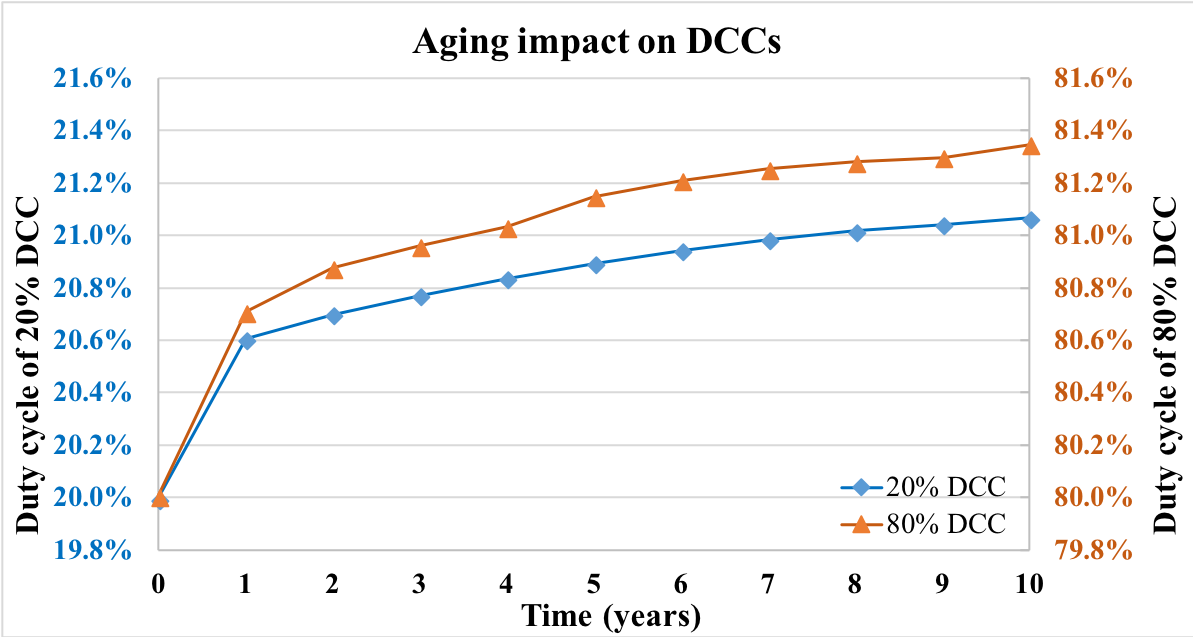
\includegraphics[width=0.9\columnwidth]{images/Aging_impacted_on_DCC.png} 
    \caption{Aging impact on 20\%/80\% DCC under BTI}
    \label{fig:exp4}
\end{figure}

Figure~\ref{fig:exp4} shows the change in the duty cycle of a 20\%/80\% DCC over 10-year aging. The y axis on the left represents the duty cycle of a 20\% DCC, and the one on the right represents the duty cycle of an 80\% DCC. As it can be seen, the growth in both cases are marginal: $20\% \to 21.07\%$ for a 20\% DCC and $80\% \to 81.35\%$ for an 80\% DCC, which in turn should not affect the benefit of our proposed framework significantly.


\section{Discussion: Depth Boundary for DCC Deployment}
\begin{figure}
    \centering
    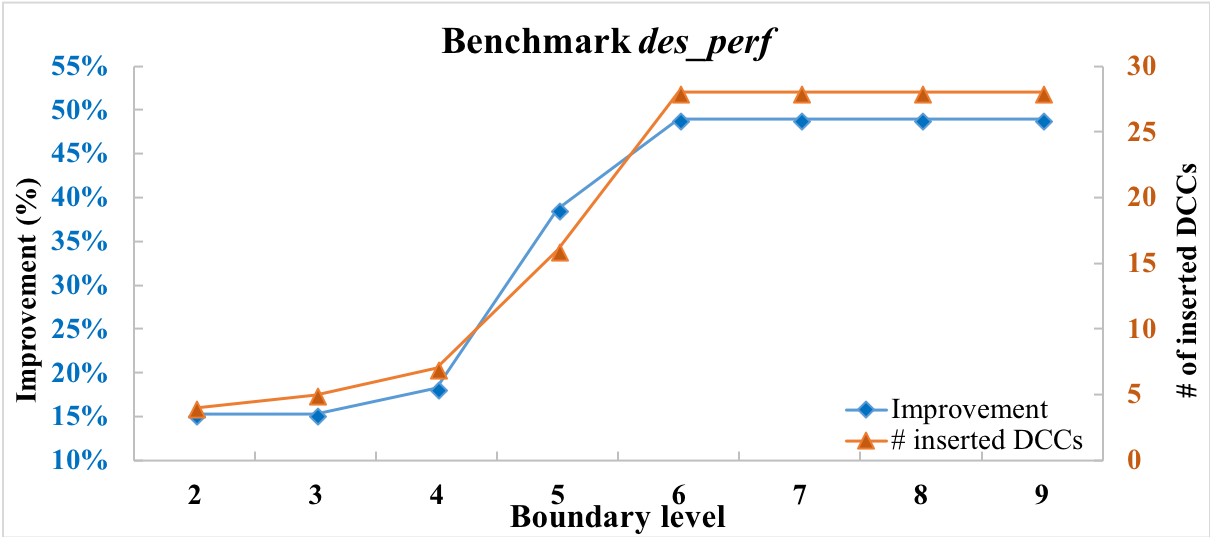
\includegraphics[width=0.9\columnwidth]{images/Boundary_level_vs_improvement.png} 
    \caption{Improvement/Cost versus clock tree level considered}
    \label{fig:boundary}
\end{figure}

As mentioned in Section~\ref{sec:framework}, inserting DCCs deep in the clock tree is less effective. For benchmark \textit{des\_perf}, we considered the deployment of DCCs at the upper half of the clock tree (i.e., level 1 to 5) and achieved 38.66\% improvement in terms of aging tolerance. As demonstrated in Figure~\ref{fig:boundary}, if we expand the boundary of DCC deployment from level 1 in the clock tree to level 10 progressively, we can gain a considerable improvement from level 1 to 6; however, from 7 to 10, the improvement become stagnant, but more DCCs are required.


\section{Discussion: Clock period calibrations during binary search}
\begin{figure}
    \centering
    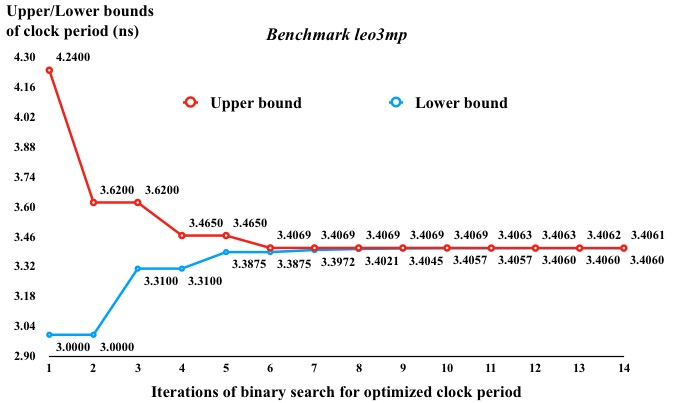
\includegraphics[width=1\columnwidth]{images/leo3mp_Tc.png} 
    \caption{Calibrations of upper/lower bounds of $T_{c}$ during iterations of binary search}
    \label{fig:Tc}
\end{figure}

It is worth reminding that, the proposed framework is based on a binary search for optimized clock period $T_{c}$, with initial two bounds of $T_{c}$ (see Section~\ref{sec:framework} or Figure~\ref{fig:flow}). During the iterations of binary search, the two bounds of $T_{c}$ are calibrated toward a convergent value, based on the satisfiability of the SAT problem, which the problem of DCC deployment and leader selection is formulated as.

Figure~\ref{fig:Tc} shows the calibrations of the two bounds of $T_{c}$ for benchmark $leo3mp$, during iterations of binary search. The X-axis denotes the iteration times of binary search and Y-axis denotes the upper (red line) and lower bounds (blue line) of $T_{c}$. In the 1\textsuperscript{st} iteration of binary search, the upper bound and lower bound are set to 4.24ns and 3ns, respectively. Then, we use the mean value of two bounds (i.e., 3.62ns) to generate the associated CNF clauses based on timing constraints. The CNF clauses are satisfiable from the output of SAT solver, implying that we can explore more lower clock period (i.e., better aging tolerance) by moving the upper bound to 3.62ns, such that the resulting upper and lower bounds are 3.62ns and 3ns, respectively. Then, in the 2\textsuperscript{ed} iteration, we use the mean value of two bounds (i.e., 3.31ns) to generate associated CNF clauses, which are unsatisfiable from the output of SAT solver, implying the clock period 3.31ns is too low, such that we move the lower bound to 3.31ns. In this manner, the upper and lower bounds will converge toward 3.4061ns. The convergent value of 3.406ns is the optimized clock period for aging tolerance.

As observed in Figure~\ref{fig:Tc}, we totally use 14 iterations of binary search to reach the convergent value of $T_{c}$, with the accuracy of third digit below the decimal point. If we degrade the accuracy from the third digit to the second digit, we only need 8 iterations. In this manner, we can nearly save half of the runtime. 


\section{Discussion: Clause count variations during binary search}
\begin{figure}
    \centering
    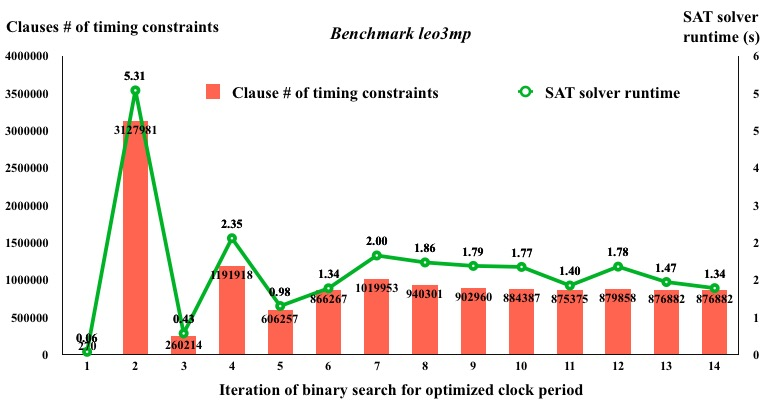
\includegraphics[width=1\columnwidth]{images/leo3mp_Cl.png} %ACM
    \caption{Variations of CNF clause count during iterations of binary search}
    \label{fig:Cl}
\end{figure}

During binary search, we generate associated CNF clauses based on timing constraints, i.e., inequality Equation~(\ref{eq:tsu}) and (\ref{eq:th}). 
As the two bounds of $T_{c}$ vary during binary search, the clause count changes because $T_{c}$ is one timing variable in Equation~(\ref{eq:tsu}) and (\ref{eq:th}). 

Figure~\ref{fig:Cl} plots the clause count in each iteration of binary search, for benchmark $leo3mp$. The clause count depends on the mean value of two bounds of $T_{c}$. If the mean value is too low/high, more/less DCC deployment and more/less leader selection will violate the timing constraints, resulting in more/less associated CNF clauses. For instance, in the 2\textsuperscript{nd} iteration of binary search for benchmark $leo3mp$, the mean value of two bounds is low (3.31ns, see Figure~\ref{fig:Tc}), resulting in large clause count (312798 clauses, see Figure~\ref{fig:Cl}). Thanks to the SAT solver such as MiniSat, we can efficiently solve the SAT problem, which is formulated as CNF clauses, at the cost of less than 10s in each iteration (at most 5.31s for benchmark $leo3mp$).


%In each iteration of binary search, we generate associated CNF clauses based on timing constraints (Section~\ref{sec:VTA:timing}), according to the mean value of two bounds of $T_{c}$. Since the values of two bounds vary in each iteration, the count of CNF clauses changes. Figure~\ref{fig:Cl} plots the clause count in each iteration of binary search, for benchmark $leo3mp$. The clause count strongly depends on the mean value of two bounds of $T_{c}$. If the mean value is too low/high, more/less DCC deployment and more/less leader selection will violate the timing constraints, resulting in more/less associated CNF clauses. For instance, in the 2\textsuperscript{nd} iteration of binary search for benchmark $leo3mp$, the mean value of two bounds is low (3.31ns, see Figure~\ref{fig:Tc}), resulting in large clause count (312798 clauses, see Figure~\ref{fig:Cl}). Thanks to the SAT solver such as MiniSat, we can efficiently solve the SAT problem, at the cost of less than 10s in each iteration.






